% Template LaTeX document for CSSR4A Deliverables
% Adapted from documents prepared by EPFL for the RobotCub project
% and subsequently by the University of Skövde for the DREAM project
%
% DV 28/06/2023

\documentclass{CSSRforAfrica}

\usepackage[titletoc,title]{appendix}
\usepackage[colorlinks, urlcolor=blue, linkcolor=black, citecolor=black]{hyperref}
\usepackage{latexsym}
\usepackage{comment}
\usepackage{multirow}
\usepackage{subcaption}
\usepackage[breakable,skins,most]{tcolorbox} % Consolidated tcolorbox options
\usepackage{tabularx,colortbl}
\usepackage[tikz]{bclogo} % for boxes
\usepackage{ragged2e}
\usepackage{dirtree}
\usepackage{listings}
\usepackage{textcomp}
\usepackage{natbib}
\usepackage{url}
\usepackage{graphicx}
\usepackage{array}
\usepackage{longtable}
\usepackage{makecell} 
\usepackage{forest}
\usepackage{hyperref}
\usepackage{graphicx}
\usepackage{pdfpages}
\usepackage{pdfpages}
\usepackage{float}



\usepackage{tikz}
\usetikzlibrary{positioning,shapes,arrows,fit,backgrounds}

% Required Packages
\usepackage{xcolor} % For colors
\usepackage{tcolorbox} % For creating styled boxes
\usepackage{listings} % For code formatting

% Define a custom style for bash code
\lstdefinestyle{linuxbashstyle}{
    language=bash,
    backgroundcolor=\color{gray!10}, % Light gray background
    basicstyle=\ttfamily\small, % Monospaced font
    keywordstyle=\color{blue}, % Color for bash keywords
    stringstyle=\color{green}, % Color for strings
    commentstyle=\color{red}, % Color for comments
    showstringspaces=false, % Do not display spaces in strings
    breaklines=true, % Wrap lines
    columns=fullflexible, % Adjust column width
    frame=single, % Box around the code
    rulecolor=\color{gray!10}, % Border color
}

% Create a reusable command for adding code with comments
\newcommand{\stepwithcode}[2]{%
    \noindent\textbf{#1}
    \lstset{style=linuxbashstyle}
    \begin{lstlisting}
## #2
    \end{lstlisting}
}





\lstset{upquote=true}
\renewcommand{\DTstyle}{\footnotesize\sffamily}

%%%%%%%%%%%%%%%%%%%%%%%%%%%%%%%%%
\captionsetup[figure]{format=hang}
\definecolor{codegreen}{rgb}{0,0.6,0}
\definecolor{greenyellow}{rgb}{0.8, 0.7, 0.10}
\definecolor{backcolour}{rgb}{0.95,0.95,0.95} 

\lstdefinestyle{withoutNumbering}{
    backgroundcolor=\color{backcolour},   
    commentstyle=\color{codegreen},
    keywordstyle=\color{magenta},
    stringstyle=\color{codepurple},
    basicstyle=\ttfamily\small,
    breakatwhitespace=false,         
    breaklines=true,                 
    captionpos=b,                    
    keepspaces=true,                 
    showspaces=false,                
    showstringspaces=false,
    showtabs=false,                  
    tabsize=2
}
%%%%%%%%%%%%%%%%%%%%%%%%%%%%%%%%%%%%%%%%%%%%%%%%%%%
\newcommand{\blank}{~\\}
\newcommand{\checkbox}{{~~~~~~~\leavevmode \put(-7,-1.5){  \huge $\Box$  }}}

\begin{document}
\input{epsf}

%%
%% SHOULD NOT NEED TO BE CHANGED BEFORE THIS POINT
%% ------------------------------------------------
%%

\deliverable{D5.2}                              % REPLACE with correct number
\title{D5.2  Animate Behaviour Subsystem}               % REPLACE with correct title

\leadpartner{Carnegie Mellon University Africa} % REPLACE with partner name: Carnegie Mellon University Africa or The University of the Witwatersrand
\partner{}                                      

\revision{1.1}                          % REPLACE with correct version number
\deliverabledate{31/03/2024	}   		%I used this date from the website
\submissiondate{21/12/2024}  			% REPLACE with date
\revisiondate{23/01/2025}                      % REPLACE with date
\disseminationlevel{PU}
\responsible{Eyerusalem Mamuye Birhan}      		% REPLACE with correct  name


%%
%% Create the title page
%%

\maketitle

\section*{Executive Summary}
%==============================================================
Deliverable D5.2 of the Animate behaviour Subsystem, part of the CSSR4Africa project, aims to enhance the robot’s lifelike appearance through random movements. This deliverable seeks to create an engaging and interactive experience by implementing a robust ROS-based module named  \texttt{animateBehaviour}. The module controls the actuators of the Pepper robot to perform random, subtle body movements, flex its hands, and slightly rotate its base along the Z-axis. All joints, except for \textit{headYaw} and \textit{headPitch}, are actuated to generate these motions.\\[1em]
The \texttt{animateBehaviour} node generates movements in a randomized pattern and advertises the \texttt{/animateBehaviour/set\_activation} service to enable or disable its operation, allowing dynamic activation and deactivation. This deliverable includes a comprehensive report on the development process, covering the refinement of initial requirements, definition of functional characteristics, and systematic development procedures. Additionally, it provides a detailed user guide with instructions on the code structure, configuration file parameters, and selective invocation of animate behaviours—body movement, hand flexing, and base rotation.\\[1em]
Overall, this report provides a comprehensive overview of the development and implementation of the animate behaviour subsystem. It details the functional specifications and technical design of the \texttt{animateBehaviour} ROS node.

\label{executive_summary}

%\graphicspath{{./figs/}}
\pagebreak
\tableofcontents

\newpage

\pagebreak

\section{Introduction}
Deliverable D5.2 focuses on the development and implementation of the \texttt{animateBehaviour} subsystem, a component designed to enhance the lifelike appearance of Pepper robot. By periodically actuating its joints in random patterns, this subsystem aims to give the robot more natural and dynamic movements. This deliverable is part of Task 5.2, which aims to provide both functional software and comprehensive documentation detailing the various stages of the software development process.\\[1em]
The animateBehaviour module is a ROS-based system that controls pepper's actuators.  It enables the robot to perform subtle body movements, flex its hands, and slightly rotate its base along the Z-axis. This movement is achieved by actuating all joints except for headYaw and headPitch, which are managed by the Attention subsystem. By generating movements in a randomized pattern, the module creates a natural and lifelike appearance for the robot.\\[1em]
A key feature of the animateBehaviour module is its dynamic activation and deactivation capability via the service \texttt{/animateBehaviour/set\_activation}. The module's operation is governed by a configuration file, \texttt{animateBehaviourConfiguration.ini}, which specifies crucial parameters such as the platform (robot or simulator), type of animate behaviour, range of movement, and topic name of the actuators. This configuration ensures compatibility with both the physical Pepper robot and a simulator. Additionally, the module includes a verbose mode that provides detailed diagnostic information, which is useful for debugging and monitoring the system’s performance.\\[1em]
This report outlines the detailed specifications of the animateBehaviour module, covering interface design, module design, and execution of the animate behaviour. The subsequent sections will delve into each aspect comprehensively, ensuring that all components and functionalities are clearly explained and documented.\\[1em]
%%%%%%%%%%%%%%%%%%%%%%%%%%%%%%%%%%%%%%%%%%%%%%%%%%%%%%%%%%%%%%%%%%%%%%%%%%%%%%%%%%%%%%%%%%%%%%%%%%%%%%%%%%%%%%%%
\newpage
\section{Requirements Definition}
The animateBehaviour module has been designed and implemented to enhance the lifelike appearance of the Pepper robot by actuating its joints periodically in random patterns. This section details the functional requirements that have been met to achieve this objective.
\subsubsection*{Randomized Joint Movements}
The primary function of the animateBehaviour module is to actuate the robot joints periodically in a random pattern. This functionality aims to simulate natural movements by keeping the joint angles close to their default home positions. The randomization ensures that the movements are not repetitive, contributing to a more realistic appearance of the robot.
\subsubsection*{Selective behaviour Invocation}
The module supports the selective invocation of any of the three types of animate behaviour. If no specific behaviour is selected, all three behaviours will be invoked using \texttt{All}. The supported behaviours are:
\begin{itemize}
    \item Body Movement: Subtle movements of the robot's body.
    \item Hand Flex: Flexing movements of the robot's hands.
    \item Base Rotation: Slight rotation of the robot's base along the Z-axis.
    \item All: All three behaviours will be invoked
\end{itemize}
This feature allows for targeted animations depending on the context, enhancing the flexibility and applicability of the module. 
\subsubsection*{Dynamic Activation/Deactivation}
To manage the operational state of the module, a service has been implemented to provide dynamic activation and deactivation. 
\subsubsection*{Configuration Flexibility}
The animateBehaviour module has been implemented to ensure compatibility with both the physical Pepper robot and a simulator, allowing for development, testing, and deployment across various platforms. Its operation is governed by a configuration file, \texttt{animateBehaviourConfiguration.ini}, which specifies key parameters such as platform, type of animate behaviour, range of movement, and topic names for actuators, enabling easy adaptation to different environments without altering the core codebase. A verbose mode is included to provide detailed diagnostic information, which is useful for debugging and monitoring the ROS node performance by outputting detailed logs of operations, movement commands, status updates, and errors.

\newpage
%%%%%%%%%%%%%%%%%%%%%%%%%%%%%%%%%%%%%%%%%%%%%%%%%%%%%%%%%%%%%%%%%%%%%%%%%%%%%%%%%%%%%%%%%%%%%%%%%%%%%%%%%%%%%%%%
\section{Module Specifications}
The animate behaviour module implements three core movement types to create lifelike animations: flexible hand movements, subtle body movements, and base rotation. All movements are periodic and follow a random pattern, with the random positions close to the default home position.
\subsection*{Generating Random Movements}
\label{sec:math_random_movements}
To calculate the random position centered on the home position, two percentage values are used: the \texttt{selected range} and the \texttt{maximum range}. The \texttt{selected range} is the same for all actuators, while the \texttt{maximum range} varies between them.\\
\begin{itemize}
    \item \textbf{Arm Actuators}: The \texttt{armMaximumRange} is a list of five values defined in the configuration. Each value corresponds to a specific joint as follows:
    \begin{itemize}
        \item \texttt{RShoulderPitch}
        \item \texttt{ShoulderRoll}
        \item \texttt{ElbowRoll}
        \item \texttt{ElbowYaw}
        \item \texttt{WristYaw}
    \end{itemize}
    For example, the default maximum range values for the arm are \texttt{0.2, 0.2, 0.2, 0.35, 0.2}, corresponding to the above joints respectively.

    \item \textbf{Hand Actuators}: The \texttt{handMaximumRange} is a single value defined in the configuration, and it applies to both the left and right hands. This value corresponds to the hand joint. For example, in the configuration file, the preferred value is set to \texttt{0.7}.
 
    \begin{itemize}
        \item \texttt{Hand}
    \end{itemize}

    \begin{tcolorbox}[colback=yellow!20,colframe=yellow!50!black,title=NOTE]
The hand actuator implementation is restricted to the physical robot system and does not function in simulation environments. For implementation details, consult the \href{https://cssr4africa.github.io/deliverables/CSSR4Africa_Deliverable_D5.1.pdf}{Actuator Test} documentation. Flexible hand movement is achieved through coordinated control of the elbow roll and wrist yaw joints, operating within defined position constraints.
\end{tcolorbox}
    \item \textbf{Leg Actuators}: The \texttt{legMaximumRange} is a list of three values defined in the configuration. Each value corresponds to a specific joint as follows:
    \begin{itemize}
        \item \texttt{HipPitch}
        \item \texttt{HipRoll}
        \item \texttt{KneePitch}
    \end{itemize}
    For example, the default maximum range values for the leg are \texttt{0.1, 0.1, 0.08}, corresponding to the above joints respectively.

   \item \textbf{Rotation Actuators}: The \texttt{rotMaximumRange} is a single value defined in the configuration. This value corresponds to the rotation joint. For example, in the configuration file, the default value is set to \texttt{0.3}.
    \begin{itemize}
        \item \texttt{Wheel}
    \end{itemize}
\end{itemize}
Using the two main percentage values set above, the steps to calculate the random position are described in Table~\ref{table} step by step.
\begin{table}[H]
\centering
\caption{Step-by-step calculation of random position.}
\renewcommand{\arraystretch}{1.3}
\begin{tabularx}{\textwidth}{|>{\raggedright\arraybackslash}X|>{\raggedright\arraybackslash}X|}
\hline
\rowcolor{white}
\textbf{Step [Variable]} & \textbf{Mathematical Formula} \\
\hline
\rowcolor{white}
1. Full Range [FR] & \textcolor{brown}{$FR = MaxPosition - MinPosition$} \\
\hline
\rowcolor{white}
2. Maximum Range Offset [MRO] & \textcolor{brown}{$MRO = FR \times MaxRangePercentage$} \\
\hline
\rowcolor{white}
3. Selected Range Offset [SRO] & \textcolor{brown}{$SRO = (MRO \times SelectedRangePercentage) / 2$} \\
\hline
\rowcolor{white}
4a. Upper Position Bound [UB] & \textcolor{brown}{$UB = \min(HomePosition + SRO, MaxPosition)$} \\
\hline
\rowcolor{white}
4b. Lower Position Bound [LB] & \textcolor{brown}{$LB = \max(HomePosition - SRO, MinPosition)$} \\
\hline
\rowcolor{white}
5. Random Position [RP] & \textcolor{brown}{$RP \in [LB, UB]$} \\
\hline
\end{tabularx}
\label{table}
\end{table}

\begin{tcolorbox}[colback=yellow!20,colframe=yellow!50!black,title=NOTE]
The algorithm generates random positions for actuators, and each position is constrained such that both the maximum range percentage and the selected range percentage must be between 0 and 1. Furthermore, the home position must be between the minimum and maximum positions ($MinPosition \leq HomePosition \leq MaxPosition$). The final random position is generated within these bounds ($LB \leq RP \leq UB$).
\end{tcolorbox}
\noindent To achieve smooth movement patterns, instead of generating and moving to individual target positions, the system uses a list of pre-generated random positions. For all joints except the leg, a list of random positions (configurable via \texttt{numPoints}) is generated. In the configuration file, the default value is set to 100, and the actuators move through this list continuously. However, leg joints (HipPitch, HipRoll, KneePitch) require a different approach due to their movement characteristics.
For leg joints, continuous movement through 100 positions would result in excessive motion without sufficient pauses. The solution implements a chunked pattern approach, where the total positions (\texttt{numPoints} = 100) are divided into chunks. The chunk size is determined by two configuration parameters: \texttt{numPoints} and \texttt{legRepeatFactor} (set to 8). The \texttt{legRepeatFactor} determines how many random positions (\texttt{numPointsLeg} set to 2) will be executed while other joints complete their 100-position sequence.\\[1em]
Each chunk follows a specific pattern: the first two positions are random movements, followed by home positions for the remainder of the chunk (about 10 home positions, as \texttt{chunkSize} = \texttt{numPoints} / \texttt{legRepeatFactor} = 100 / 8 = 12). This creates a movement pattern where the leg moves to two random positions, stays at the home position for a time interval, and then moves to the next set of random positions. This cycle continues through all 8 chunks, creating a more controlled and rhythmic movement pattern suitable for leg joints.\\[1em]
\newpage
\noindent Pattern Structure:
\begin{verbatim}
Total Positions (numPoints) = 100
Leg Repeat Factor = 8
Random Positions per chunk (numPointsLeg) = 2
Chunk Size = numPoints/legRepeatFactor = 100/8 = 12 

+-------------------+  +-------------------+  +-------------------+
| R R H H H H H ...|  | R R H H H H H ...|  | R R H H H H H ...| ...
+-------------------+  +-------------------+  +-------------------+
 ^ ^       ^
 | |       |
 2 Random  10 Home positions

\end{verbatim}

\begin{tcolorbox}[colback=yellow!20,colframe=yellow!50!black,title=NOTE]
If the chunk size is not a whole number, the total leg positions might not sum up to 100. In such cases, the remaining positions are filled with the home position. For example, if there are 96 positions, the last 4 will be set to the home position. To avoid this, use leg repeater factors that divide evenly into 100.
\end{tcolorbox}

%%%%%%%%%%%%%%%%%%%%%%%%%%%%%%%%%%%%%%%%%%%%%%%%%%%%%%%%%%%%%%%%%%%%%%%%%%%%%%%%%%%%%%%%%%%%%%%%%%%%%%%%%%%%%%%%%%%%%%%%%%%
\newpage
\section{Implementation}
\subsection*{File Organization and Its Purposes}  
The \texttt{animateBehaviour} directory is organized to include configuration files, data, header files, source code, services, \texttt{README.md}, and \texttt{CMakeLists.txt}, as illustrated in Figure \ref{fig:dir-structure}. 
\\[1em] 
The \texttt{config} folder contains configuration settings, such as \texttt{animateBehaviourConfigurati}\\
\texttt{on.ini}, and defines parameters for behaviour customization. The \texttt{data} folder holds critical resources, including \texttt{pepperTopics.dat} and \texttt{simulatorTopics.dat}, which provide topic mappings for communication with the Pepper robot or its simulator. The \texttt{include/animate\_behaviour} folder contains header files, such as \texttt{animateBehaviourInterface.h}, that define interfaces and declarations used throughout the module.\\[1em] 
The \texttt{src} folder houses implementation files, such as \texttt{animateBehaviourApplication.cpp} for application logic and \texttt{animateBehaviourImplementation.cpp} for detailed functional execution. Additionally, the \texttt{README.md} file provides documentation for understanding and using the module, while the \texttt{CMakeLists.txt} file manages the build system configuration. The directory also includes services to enable and disable the node, allowing dynamic control of its activation.
\begin{figure}[h]
\begin{center}
\begin{forest}
for tree={
  font=\small\ttfamily,
  grow'=0,
  child anchor=west,
  parent anchor=south,
  anchor=west,
  calign=first,
  inner sep=1pt,
  edge path={
    \noexpand\path [draw, \forestoption{edge}]
    (!u.south west) +(4pt,0) |- node[fill,inner sep=1pt] {} (.child anchor)\forestoption{edge label};
  },
  before typesetting nodes={
    if n=1
      {insert before={[,phantom]}}
      {}
  },
  fit=band,
  before computing xy={l=10pt},
}
[CSSR\_SYSTEM
  [animateBehaviour
    [config [animateBehaviourConfiguration.ini]]
    [data
      [animateBehaviourLogFile.log]
      [pepperTopics.dat]
      [simulatorTopics.dat]]
    [include
      [animate\_behaviour [animateBehaviourInterface.h]]]
    [launch]
    [src
      [animateBehaviourApplication.cpp]
      [animateBehaviourImplementation.cpp]]
    [srv [setActivation.srv]]]
  [CMakeLists.txt]
  [CSSR4AfricaLogo.svg]
  [README.md]]
\end{forest}
\end{center}
\caption{Directory structure for the animate behaviour ROS package}
\label{fig:dir-structure}
\end{figure}

%%%%%%%%%%%%%%%%%%%%%%%%%%%%%%%%%%%%%%%%%%%%%%
\subsection*{Configuration File}
\label{sec:configuration file}
The operation of the \texttt{animateBehaviour} node is determined by the contents of a configuration file, \texttt{animateBehaviourConfiguration.ini}, which contains a list of key-value pairs as shown in the table below.
\begin{longtable}{|>{\raggedright\arraybackslash}p{0.23\textwidth}|>{\raggedright\arraybackslash}p{0.7\textwidth}|}
    \caption{Configuration parameters for the animate behaviour module.} 
    \label{tab:config_params} \\
    \hline
    \rowcolor{gray!30}
    \textbf{Key} & \textbf{Description} \\ \hline
    \endhead % header for subsequent pages
    
    \texttt{platform} & Specifies the target platform to be used, which can be set to either \texttt{simulator} or \texttt{robot}. \\ \hline
    
    \texttt{robotTopics} & Specifies the name of the robot topics file. The robot topics file contains the list of topics for the robot. \\ \hline
    
    \texttt{simulatorTopics} & Specifies the name of the simulator topics file. The simulator topics file contains a list of simulator topics. \\ \hline

    \texttt{verboseMode} & If it is set to \texttt{false}, the terminal will print the configuration values, copyright notice, startup messages, configuration values, and heartbeat messages. If there is an error, the error message will also be displayed. When the verbose mode is set to \texttt{true}, additional \texttt{ROSINFO} messages used for debugging will be printed.\\ \hline
    
    \texttt{rotMaximumRange} & Used in the \texttt{calculateAngularVelocityZ()} function to determine the maximum rotation range for base movements. The value \texttt{0.3} means 30\% of the maximum possible angular velocity will be used, and it is multiplied by the full range to limit how fast the robot can rotate. You can increase this value up to \texttt{0.5} for more noticeable rotations, but values above this might make the robot unstable.
    \\ \hline
    
    \texttt{selectedRange} & The \texttt{selectedRange} parameter acts as a global scaling factor for all movements, except rotation. Set at \texttt{0.5} (50\%), it provides a good balance between visible movement and stability. You can adjust this value between \texttt{0.3} and \texttt{0.7}; lower values create more subtle movements, while higher values make movements more noticeable.
    \\ \hline
    
    \texttt{armMaximumRange} & The \texttt{armMaximumRange} uses five values for different arm joints: \texttt{0.2}, \texttt{0.2}, \texttt{0.2}, \texttt{0.35}, and \texttt{0.2} for \texttt{ShoulderPitch}, \texttt{ShoulderRoll}, \texttt{LElbowRoll}, \texttt{LElbowYaw}, and \texttt{LWristYaw}, respectively. The slightly higher value (\texttt{0.35}) for the elbow yaw allows more natural elbow movement. Keep the shoulder values (the first two numbers) lower for stability.
    \\ \hline
    
    \texttt{handMaximumRange} & The \texttt{handMaximumRange} set at \texttt{0.7} allows significant joint \texttt{hand} opening and closing. You can adjust this value between \texttt{0.5} and \texttt{0.8}, depending on how expressive you want the hand gestures to be.
    \\ \hline
    
    \texttt{legMaximumRange} & The \texttt{legMaximumRange} values \texttt{(0.1, 0.1, 0.08)} for \texttt{HipPitch}, \texttt{HipRoll}, and \texttt{KneePitch}, respectively, are intentionally conservative to maintain balance. The hip joints (the first two values) are set at 10\% range, while the knee is slightly more restricted at 8\%. It is recommended not to exceed \texttt{0.15} for any leg joint to prevent stability issues.
    \\ \hline
    
    \texttt{gestureDuration} & The \texttt{gestureDuration} parameter (currently set to \texttt{1.0} second) is a timing control that determines how long the robot takes to move between each randomly generated position. When the system calculates random positions for arms, hands, or legs, these positions become waypoints in a movement trajectory, and the \texttt{gestureDuration} specifies the time allocated to travel between each waypoint. Setting a lower duration value (like \texttt{0.5}) creates faster but potentially more abrupt movements, while higher values (like \texttt{2.0}) result in slower motions. The preferred value is \texttt{1.0}, which provides balanced timing to create subtle body movement.
    \\ \hline
    
    \texttt{numPoints} & The \texttt{numPoints} parameter (preferred value set to \texttt{100}) determines the total number of random positions generated for arm and hand movements. The purpose is to create a set of random positions, which are passed as a single trajectory. This approach helps reduce jerks, as it smooths the transitions between each set of \texttt{100} joint positions.
    \\ \hline
    
    \texttt{numPointsLeg} & The \texttt{numPointsLeg} parameter (preferred value set to \texttt{2}) determines the number of random positions generated for leg movements within each repetition cycle. The purpose is to create a small set of random positions, which are then repeated based on the \texttt{legRepeatFactor} value. This approach helps maintain stability by using minimal leg movements while still creating subtle motions through controlled repetition.
    \\ \hline
    
    \texttt{legRepeatFactor} & The \texttt{legRepeatFactor} parameter (preferred value set to \texttt{8}) determines how many times the leg movements generated by \texttt{numPointsLeg} are repeated. When \texttt{legRepeatFactor} is set to \texttt{8}, the system takes the \texttt{2} generated positions and repeats them \texttt{8} times, creating a total of \texttt{16} movement points that run parallel to the \texttt{100} points generated for arm and hand movements. This synchronized approach ensures coordinated full-body animation while maintaining stable leg motions.
\\ \hline

\end{longtable}


\subsection*{Input File}
This node does not read from an input data file.

\subsection*{Output Data File}
This node writes a log file to \texttt{animateBehaviourLogFile.log} as output, which will be used as input information for unit test cases.

\subsection*{Topics Subscribed}
This node does not subscribe to any topics.
\subsection*{Topics Published}
This node publishes actuator topics listed in Table \ref{tab:topics_actuators_platforms}, which are specified in the configuration file using the key-value pairs provided in \texttt{pepperTopics.dat} and \texttt{simulatorTopics.dat}. These \texttt{.dat} files are stored in the \texttt{data} section of the \texttt{animateBehaviour} node.
\\[1em]
When \texttt{pepperTopics.dat} is set in the configuration file, the node uses the topics defined in \texttt{pepperTopics.dat}, which are published in the physical actuators of the robot. Similarly, when \texttt{simulatorTopics.dat} is set in the configuration file, the node publishes to the topics specified in \texttt{simulatorTopics.dat}, enabling communication with the simulator.
% Use custom column type to ensure wrapping
%%%%%%%%%%%%%%%%%%%%%%%%%%%%%%%%%%%%%%%%%%%%%%%%%%%%%%%%%%%%%%%%%%%%%%%%%%%%%%%%%%%%%%%%%%%%%%%%%%%%%%%%%%%%
\newcolumntype{P}[1]{>{\raggedright\arraybackslash}p{#1}}
\begin{longtable}{|>{\raggedright\arraybackslash}P{0.48\textwidth}|>{\raggedright\arraybackslash}P{0.3\textwidth}|>{\raggedright\arraybackslash}P{0.17\textwidth}|}
    \caption{Topics, Actuators, and Platforms} 
    \label{tab:topics_actuators_platforms} \\
    \hline
    \rowcolor{gray!30}
    \textbf{Topic} & \textbf{Actuator} & \textbf{Platform} \\ 
    \hline
    \endfirsthead
    \hline
    \rowcolor{gray!30}
    \textbf{Topic} & \textbf{Actuator} & \textbf{Platform} \\ 
    \hline
    \endhead
    \hline \multicolumn{3}{|r|}{\textit{Continued on the next page}} \\ 
    \hline
    \endfoot
    \hline
    \endlastfoot

    % Pepper Topics Data
    \makecell[l]{\texttt{/pepper\_dcm/RightHand\_controller/} \\ \texttt{follow\_joint\_trajectory}} & RHand & Physical robot \\ \hline
    \makecell[l]{\texttt{/pepper\_dcm/LeftHand\_controller/} \\ \texttt{follow\_joint\_trajectory}} & LHand & Physical robot \\ \hline
    \makecell[l]{\texttt{/pepper\_dcm/RightArm\_controller/} \\ \texttt{follow\_joint\_trajectory}} & RShoulderPitch, RShoulderRoll, RElbowYaw, RElbowRoll, RWristYaw & Physical robot \\ \hline
    \makecell[l]{\texttt{/pepper\_dcm/LeftArm\_controller/} \\ \texttt{follow\_joint\_trajectory}} & LShoulderPitch, LShoulderRoll, LElbowYaw, LElbowRoll, LWristYaw & Physical robot \\ \hline
    \makecell[l]{\texttt{/pepper\_dcm/Pelvis\_controller/} \\ \texttt{follow\_joint\_trajectory}} & HipRoll, HipPitch, KneePitch & Physical robot \\ \hline
    \makecell[l]{\texttt{/pepper\_dcm/cmd\_moveto}} & Wheels & Physical robot \\ \hline

    % Simulator Topics Data
    \makecell[l]{\texttt{/pepper/RightArm\_controller/} \\ \texttt{follow\_joint\_trajectory}} & RElbowYaw, RElbowRoll & Simulator \\ \hline
    \makecell[l]{\texttt{/pepper/LeftArm\_controller/} \\ \texttt{follow\_joint\_trajectory}} & LElbowYaw, LElbowRoll & Simulator \\ \hline
    \makecell[l]{\texttt{/pepper/Pelvis\_controller/} \\ \texttt{follow\_joint\_trajectory}} & HipRoll, HipPitch, KneePitch & Simulator \\ \hline
    \makecell[l]{\texttt{/pepper/cmd\_vel}} & Wheels & Simulator \\ \hline

\end{longtable}


\subsection*{Services Supported}
This node provides and advertises a server for a service \texttt{/animateBehaviour/setActivation} to enable or disable the operation of the node, i.e., to activate or suspend the publishing of data on the actuator topics to give the appearance of an animated agent. The service defines a request field \texttt{string state} which can have a value of either ``enabled'' or ``disabled''. Depending on the state value, the node will be enabled or disabled. The service returns a response value of ``1'' for success or ``0'' for failure. The service is called by the \texttt{behaviourController} node to enable or disable animated behavior as needed. The following summarizes the services supported.
\begin{longtable}{|>{\raggedright\arraybackslash}p{0.3\textwidth}|>{\raggedright\arraybackslash}p{0.2\textwidth}|>{\raggedright\arraybackslash}p{0.4\textwidth}|}
    \caption{Summary of Supported Services}
    \label{tab:services_supported}\\
    \hline
    \rowcolor{gray!30}
    \textbf{Service} & \textbf{Message Value} & \textbf{Effect} \\ \hline
    \endhead % header for subsequent pages
    \makecell[l]{\texttt{/animateBehaviour/} \\ \texttt{setActivation}} & enabled, disabled & Enable or disable animate behaviour \\ \hline
\end{longtable}

%%%%%%%%%%%%%%%%%%%%%%%%%%%%%%%%%%%%%%%%%%%%%%%%%%%%%%%%%%%%%%%%%%%%%%%%%%%%%%%%%%%%%%%%%%%%%%%%%%%%%%%%%%%%
\subsection*{Services Called}
This node does not call any services.
% Define listing styles
\lstset{
    backgroundcolor=\color{gray!20}, % Light gray background (terminal style)
    frame=single,                   % Single frame around the code
    rulecolor=\color{gray!20},      % Frame border color matches background
    basicstyle=\ttfamily\small,     % Monospace font, small size
    commentstyle=\color{green!50!black}, % Green comments
    keywordstyle=\color{blue},      % Blue keywords
    breaklines=true,                % Line breaking
    numbers=none,                   % No line numbers
    tabsize=2,                      % Tab size
    showstringspaces=false          % Do not show string spaces
}

\newpage
%%%%%%%%%%%%%%%%%%%%%%%%%%%%%%%%%%%%%%%%%%%%%%%%%%%%%%%%%%%%%%%%%%%%%%%%%%%%%%%%%%%%%%%%%%%%%%%%%%%%%%%%%%%%%%%%%%%%%%%
\section{Module Design}
The animate behaviour implementation utilizes several ROS message types to enable coordinated robot motion control. These messages facilitate joint trajectory execution, velocity commands, sensor feedback, and behaviour activation through action-based communication and service calls. Each message type serves a specific purpose in the motion control architecture, from low-level joint commands to high-level behaviour coordination.
\\[1em]
\textbf{Joint Control Messages}\\
\texttt{trajectory\_msgs::JointTrajectoryPoint}:  
It is used to specify precise positions and timing for each point in the robot's movement trajectory. It is particularly used in the \texttt{moveToListOfPos}\\
 \texttt{itions} function, where the robot needs to move through a sequence of positions in a smooth, natural-looking way.\\[1em]
\texttt{trajectory\_msgs::JointTrajectory}: The message is used in two key functions within the provided code to define the desired movement path for the robot's joints. In the \texttt{moveToPosition} function, it is used to send a single, fixed target position for the robot's joints to an action server. In the \texttt{moveToPositionBiological} function, it is used to create a more complex movement trajectory by generating a sequence of waypoints with their own joint positions and durations. This structured representation of the joint movements is essential for achieving the natural-looking and fluid animations that the robot is designed to perform.\\[1em]
\texttt{control\_msgs::FollowJointTrajectoryGoal}:  
The message is a ROS message that is used to define the parameters of joint trajectory actions. It is used in the functions \texttt{moveToPosition()} and \texttt{moveToPositionBiological()} to control the movements of the robot's arm, hand, and legs by sending trajectory goals to the action servers.
\\[1em]
\textbf{Base Motion Control Messages}\\
\texttt{geometry\_msgs::Twist}:  
The message type is a ROS message used to represent velocity commands with both linear and angular components, and it is used in the function \texttt{rotationBaseShift()} to control the robot's base rotation. Specifically, the angular velocity values along the z-axis are assigned to \texttt{twist.angular.z} and published using \texttt{velPub.publish(twist)}, allowing the robot to execute controlled rotational movements.
\\[1em]
\textbf{Action and Service Control Messages}\\
\texttt{actionlib::SimpleClientGoalState}:  
It is a state tracking message that monitors the execution status of action goals through states such as PENDING, ACTIVE, and SUCCEEDED. Provides essential feedback for coordinating robot movements and implementing error handling.
\\[1em]
\texttt{cssr\_system::setActivation}:  
It is a custom service message type used in the function \texttt{setActivation()} to enable or disable the animate behaviour system in the CSSR system. Implements a simple request-response pattern, where requests specify the desired state (``enabled" or ``disabled"), and responses indicate success or failure. This message type ensures safe and controlled activation or deactivation of robot behaviours, providing effective control over the animation state.

\newpage
%%%%%%%%%%%%%%%%%%%%%%%%%%%%%%%%%%%%%%%%%%%%%%%%%%%%%%%%%%%
\section{Executing the Animate behaviour}
To activate the node, it is essential to first understand the key aspects of the animate behaviour. There are three behaviours in this node: hands and rotation. These values are configured in the settings, as detailed in Table \ref{tab:config_params}. To further understand the random positions calculated for each joint, refer to the mathematical details explained in Section \ref{sec:math_random_movements}. This node provides and advertises a server for the service \texttt{/animateBehaviour/set\_activation}
 to enable or disable the operation of the node. The service accepts a value of \texttt{"enabled"} or \texttt{"disabled"}. Depending on the string value provided, \texttt{animateBehaviour} will be activated or deactivated. For an explanation of additional configuration values and their functionality, refer to Section \ref{sec:configuration file}. This section outlines the detailed steps required to configure, launch and test the \texttt{Animate behaviour} node for both physical robots and simulated environments.

\subsection{Physical Robot Execution}
To execute the \texttt{Animate behaviour} node on a physical robot, follow these steps:

\subsubsection*{1. Environment Setup}
Install all necessary dependencies as per the \href{https://github.com/cssr4africa/cssr4africa/blob/main/docs/D3.3_Software_Installation_Manual.pdf}{CSSR4Africa Software Installation Manual}. Clone the repository into the robot's workspace:
Move to the source directory of the workspace:\\
\begin{lstlisting}[style=linuxbashstyle]
cd $HOME/workspace/pepper_rob_ws/src
\end{lstlisting}
Clone the CSSR4Africa software from the GitHub repository:\\
\begin{lstlisting}[style=linuxbashstyle]
git clone https://github.com/cssr4africa/cssr4africa.git
\end{lstlisting}
 Build the source files:\\
\begin{lstlisting}[style=linuxbashstyle]
cd .. && catkin_make
\end{lstlisting}
Source the environment:\\
\begin{lstlisting}[style=linuxbashstyle]
source devel/setup.bash
\end{lstlisting}
%%%%%%%%%%%%%%%%%%%%%%%%%%%%%%%%%%%%%%%%%%%%%%%%%%%%%%%%%%%%
\subsubsection*{2. Configure the Node}
The configuration file \texttt{/animateBehaviourConfiguration.ini} and preferred values are set as shown in the figure below. If you want the desired behaviour (\texttt{body}, \texttt{hands}, \texttt{rotation}, or \texttt{All}), please set the behaviour you want to run. For an explanation of each configuration value, refer to Section \ref{sec:configuration file}. Otherwise, the preferred values are the ones already set in the configuration file, as shown in Table \ref{tab:configuration_parameters}.

\begin{longtable}{|>{\raggedright\arraybackslash}P{0.48\textwidth}|>{\raggedright\arraybackslash}P{0.3\textwidth}|>{\raggedright\arraybackslash}P{0.17\textwidth}|}
    \caption{Configuration Parameters for Animate behaviour Node} 
    \label{tab:configuration_parameters} \\
    \hline
    \rowcolor{gray!30}
    \textbf{Parameter} & \textbf{Value} & \textbf{Type} \\ 
    \hline
    \endfirsthead
    \hline
    \rowcolor{gray!30}
    \textbf{Parameter} & \textbf{Value} & \textbf{Type} \\ 
    \hline
    \endhead
    \hline \multicolumn{3}{|r|}{\textit{Continued on the next page}} \\ 
    \hline
    \endfoot
    \hline
    \endlastfoot

    platform & robot & string \\
    \rowcolor{gray!10}
    behaviour & all & string \\
    simulatorTopics & simulatorTopics.dat & file \\
    \rowcolor{gray!10}
    robotTopics & pepperTopics.dat & file \\
    verboseMode & false & boolean \\
    \rowcolor{gray!10}
    rotMaximumRange & 0.3 & float \\
    selectedRange & 0.5 & float \\
    \rowcolor{gray!10}
    armMaximumRange & 0.2,0.2,0.2,0.35,0.2 & float array \\
    handMaximumRange & 0.7 & float \\
    \rowcolor{gray!10}
    legMaximumRange & 0.1,0.1,0.08 & float array \\
    gestureDuration & 1.0 & float \\
    \rowcolor{gray!10}
    numPoints & 100 & integer \\
    numPointsLeg & 2 & integer \\
    \rowcolor{gray!10}
    legRepeatFactor & 8 & integer \\
\end{longtable}

%%%%%%%%%%%%%%%%%%%%%%%%%%%%%%%%%%%%%%%
\subsubsection*{3. Launch the Node}
Move to the workspace directory:\\
\begin{lstlisting}[style=linuxbashstyle]
cd $HOME/workspace/pepper_rob_ws
\end{lstlisting}
Launch the robot:\\
\begin{lstlisting}[style=linuxbashstyle]
cd .. && roslaunch cssr_system LaunchRobot.launch \
robot_ip:=172.29.111.240 network_interface:=wlp0s20f3
\end{lstlisting}
\begin{tcolorbox}[colback=yellow!20,colframe=yellow!50!black,title=NOTE]
Ensure that the IP address \texttt{172.29.111.240} and the network interface \texttt{wlp0s20f3} are correctly set based on your robot's configuration and your computer's network interface.
\end{tcolorbox}
Open a new terminal and run the \texttt{Animate behaviour} node:\\
\begin{lstlisting}[style=linuxbashstyle]
cd .. && rosrun cssr_system animateBehaviour
\end{lstlisting}
To enable animate behaviour, open a new terminal and run the code below.\\
\begin{lstlisting}[style=linuxbashstyle]
cd .. && rosservice call /animateBehaviour/setActivation "state: 'enabled'"
\end{lstlisting}
Disable the animate behaviour service:\\
\begin{lstlisting}[style=linuxbashstyle]
rosservice call /animateBehaviour/setActivation "state: 'disabled'"
\end{lstlisting}


\subsection{Simulator Execution}
To execute the \texttt{Animate behaviour} node on a Simulator follow these steps:

\subsubsection*{1. Environment Setup}
Install all necessary dependencies as per the \href{https://github.com/cssr4africa/cssr4africa/blob/main/docs/D3.3_Software_Installation_Manual.pdf}{CSSR4Africa Software Installation Manual}. Clone the repository into the robot's workspace:
Move to the source directory of the workspace:\\
\begin{lstlisting}[style=linuxbashstyle]
cd $HOME/workspace/pepper_sim_ws/src
\end{lstlisting}
Clone the CSSR4Africa software from the GitHub repository:\\
\begin{lstlisting}[style=linuxbashstyle]
git clone https://github.com/cssr4africa/cssr4africa.git
\end{lstlisting}
 Build the source files:\\
\begin{lstlisting}[style=linuxbashstyle]
cd .. && catkin_make
\end{lstlisting}
Source the environment:\\
\begin{lstlisting}[style=linuxbashstyle]
source devel/setup.bash
\end{lstlisting}

\subsubsection*{2. Configure the Node}
Update the configuration file located at \texttt{/workspace/pepper\_sim\_ws/src/cssr4africa}\\
\texttt{/animateBehaviour/config}
\texttt{/animateBehaviourConfiguration.ini} and set the platform to \texttt{simulator} and select the desired behaviour (\texttt{body}, \texttt{hands}, \texttt{rotation}, or \texttt{All}). If you want to modify other configuration values, refer to Section \ref{sec:configuration file}. Otherwise, the preferred values are the ones already set in the configuration file.

\subsubsection*{3. Launch the Node}
Move to the workspace directory:\\
\begin{lstlisting}[style=linuxbashstyle]
cd $HOME/workspace/pepper_sim_ws
\end{lstlisting}
Launch the simulator:\\
\begin{lstlisting}[style=linuxbashstyle]
cd .. && roslaunch cssr_system LaunchSimulator.launch 
\end{lstlisting}
 Open a new terminal and run the \texttt{Animate behaviour} node:\\
\begin{lstlisting}[style=linuxbashstyle]
cd .. && rosrun cssr_system animateBehaviour
\end{lstlisting}
To enable animate behaviour, open a new terminal and run the code below.\\
\begin{lstlisting}[style=linuxbashstyle]
cd .. && rosservice call /animateBehaviour/setActivation "state: 'enabled'"
\end{lstlisting}
Disable the animate behaviour service:\\
\begin{lstlisting}[style=linuxbashstyle]
rosservice call /animateBehaviour/setActivation "state: 'disabled'"
\end{lstlisting}

\newpage
%%%%%%%%%%%%%%%%%%%%%%%%%%%%%%%%%%%%%%%%%%%%%%%%%%%%%%%%%%%
\section{Unit Test}
The unit test framework for Animate behaviour is designed to test whether the node operates as expected. It examines four cases: hand, body, rotational, and all movements combined. The framework validates the correct setup, execution, and logging of these actions in physical and simulated robot environments. Detailed logs and performance reports are generated using ROS and Google Test to measure the reliability of the Animate behaviour.
%%%%%%%%%%%%%%%%%%%%%%%%%%%%%%%%%%%%%%%%%%%%%%%%%%%%%%%%%%%%%%%%%
\subsection{File Organization and Its Purposes}
\begin{figure}[h]
\begin{center}
\begin{forest}
for tree={
  font=\small\ttfamily,
  grow'=0,
  child anchor=west,
  parent anchor=south,
  anchor=west,
  calign=first,
  inner sep=1pt,
  edge path={
    \noexpand\path [draw, \forestoption{edge}]
    (!u.south west) +(4pt,0) |- node[fill,inner sep=1pt] {} (.child anchor)\forestoption{edge label};
  },
  before typesetting nodes={
    if n=1
      {insert before={[,phantom]}}
      {}
  },
  fit=band,
  before computing xy={l=10pt},
}
[animateBehaviourTest
  [config [animateBehaviourTestConfiguration.ini]]
  [data [animateBehaviourTestOutput.dat]]
  [include
    [animateBehaviourTest [animateBehaviourTestInterface.h]]]
  [launch
    [animateBehaviourLaunchRobot.launch]
    [animateBehaviourLaunchSimulator.launch]
    [animateBehaviourLaunchTestHarness.launch]]
  [src
    [animateBehaviourTestApplication.cpp]
    [animateBehaviourTestImplementation.cpp]]
  [CMakeLists.txt]
  [CSSR4AfricaLogo.svg]
  [README.md]]
\end{forest}
\end{center}
\caption{Directory structure of the Animate behaviour Test.}
\label{fig:dir-structure-test}
\end{figure}
\noindent The directory structure of the animated behaviour test framework is organized as follows. The \texttt{src} folder contains \texttt{animateBehaviourTestApplication.cpp}, which manages the main application logic, and \texttt{animateBehaviourTestImplementation.cpp}, which provides detailed test implementations. \\[1em]
The \texttt{config} folder includes \texttt{animateBehaviourTestConfiguration.ini}, a file used to enable or disable specific tests, such as hand, body, rotation or all movements. The test results are stored in the \texttt{data} folder within the \texttt{animateBehaviourTestOutput.dat} file. The \texttt{include} directory contains the header file \texttt{animateBehaviourTestInterface.h}, which defines interfaces and utility functions. 
\\[1em]
The \texttt{launch} folder includes three ROS launch files: \texttt{animateBehaviourLaunchRobot.launch}, which launches the robot; \texttt{animateBehaviourLaunchSimulator.launch}, which launches the simulator; and \texttt{animateBehaviourLaunchTestHarness.launch}, which launches both the \texttt{animateBehaviour} and \texttt{animateBehaviourTest} nodes. Furthermore, the \texttt{README.md} file provides documentation for understanding and using the test framework, while \texttt{CMakeLists.txt} configures the build system.

\subsection*{Configuration File}
\label{sec:test configuration file}
The operation of the \texttt{animateBehaviourTest} node is determined by the contents of a configuration file, \texttt{animateBehaviourTestConfiguration.ini}, that contains a list of key-value pairs as shown in Table \ref{tab:configuration_parameters}.

%%%%%%%%%%%%%%%%%%%%%%%%%%%%%%%%%%%%%%%%%%%%%%%%%%%%%%%%%%%%%%%%%%%%%%%%%
\subsection{Test Cases and Types}
The unit tests in the animate behaviour system are implemented using Google Test (gtest), a comprehensive C++ testing framework developed by Google that provides essential testing capabilities including test fixtures, assertions, test case organization, and result reporting. The testing suite implements four primary test cases:
\begin{itemize}
    \item Hand movement testing (Test01FlexiHandanimateBehaviour)
    \item Body movement testing (Test02SubtleBodyanimateBehaviour)
    \item Rotation testing (Test03RotationanimateBehaviour)
    \item Combined movement testing (Test04AllanimateBehaviour)
\end{itemize}
Each test case inherits from a base test fixture class, animateBehaviourRobotTest, which manages test setup and teardown operations, ensuring consistent test environments and proper resource management throughout the testing process.
\\[1em]
The testing implementation utilizes Google Test's assertion system and test execution control to validate movement execution, position accuracy, and system stability. The test framework for the Animate behaviour system incorporates several key features to ensure comprehensive and reliable testing. Test configuration is managed through dedicated configuration files, allowing users to selectively activate or deactivate specific tests based on requirements. Automated reporting is an integral component of the framework, generating detailed test reports that document results and capture movement data for thorough analysis. The framework also supports continuous testing, enabling repeated test execution with user-controlled iterations to ensure consistency and robustness across multiple runs.
\subsubsection*{Class Implementation}
\textbf{animateBehaviourRobotTest:} It is a test class that inherits from \texttt{testing::Test} for unit testing of robot animate behaviour. The class is structured with two static members: \texttt{testReport} (an \texttt{ofstream} pointer for test output management) and \texttt{alert} (a boolean flag). It includes two protected methods: \texttt{SetUp()} for disabling animate behaviour before each test and \texttt{TearDown()} for cleanup and report flushing after each test. The public interface provides two static methods: \texttt{setTestReportStream()} and \texttt{getTestReportStream()} for managing test reporting. The test cases are implemented using the \texttt{TEST\_F} macro from the Google Test framework.\\
\textbf{Configuration Functions:} These are standalone helper functions that manage all configuration-related operations and it include \texttt{readbehaviourConfig()} which reads test settings from configuration files and returns them as a map, \texttt{writeConfigurationFile()} which handles writing robot configuration parameters, \texttt{writeInitialConfigurationFile()} which sets up initial behaviour configuration values, and \texttt{setConfigurationAndWriteFile()} which updates specific behaviour settings in the configuration file. These functions work together to ensure proper test configuration management and state setup before test execution.
\begin{figure}[htbp]
\centering
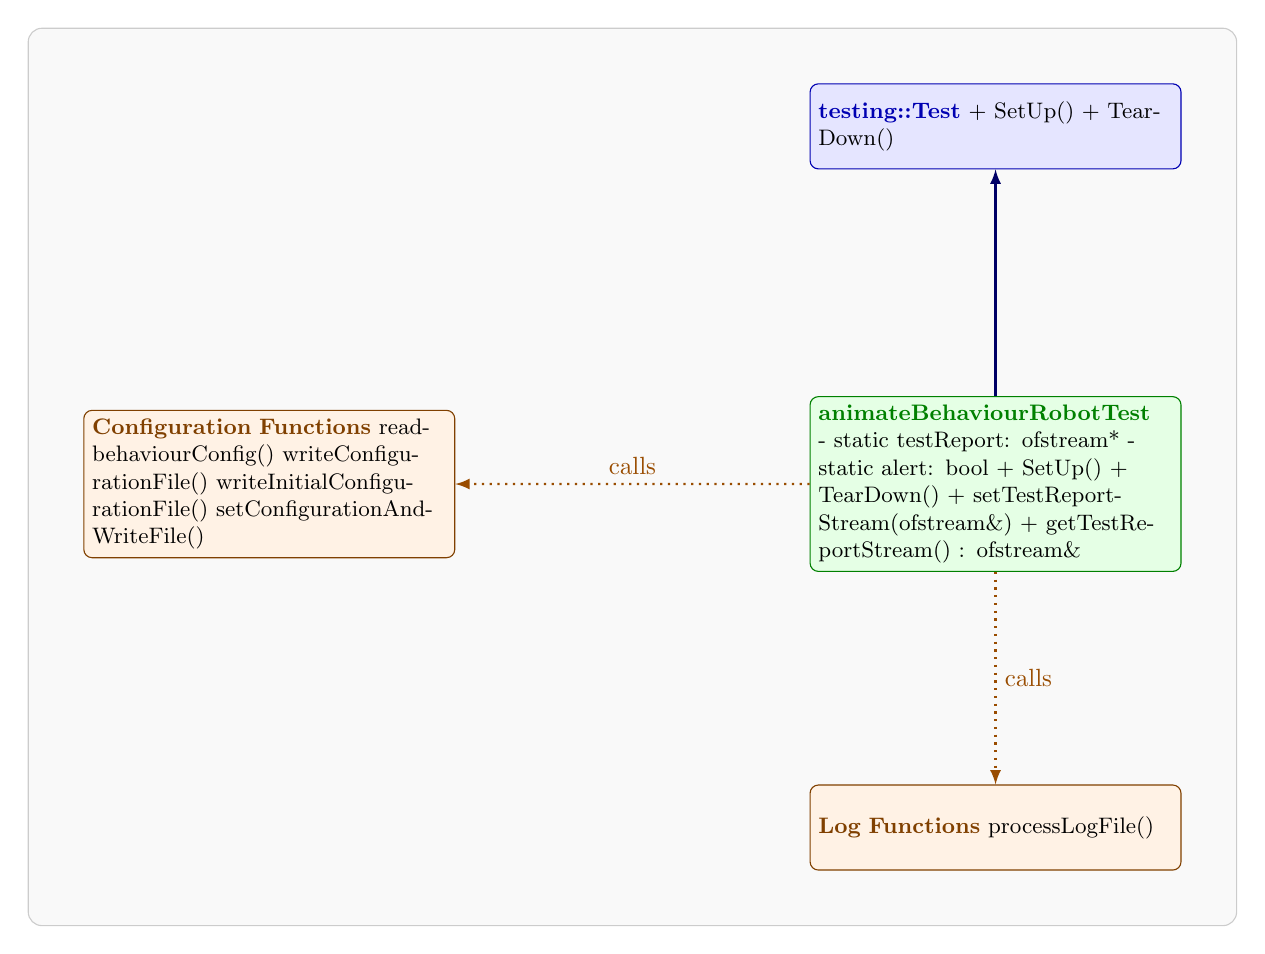
\begin{tikzpicture}[scale=0.9, transform shape,
    interface/.style={
        draw=blue!70!black,
        rectangle,
        text width=5cm,
        minimum height=1.2cm,
        align=left,
        font=\small,
        fill=blue!10,
        rounded corners=3pt
    },
    class/.style={
        draw=green!50!black,
        rectangle,
        text width=5cm,
        minimum height=1.2cm,
        align=left,
        font=\small,
        fill=green!10,
        rounded corners=3pt
    },
    functions/.style={
        draw=orange!50!black,
        rectangle,
        text width=5cm,
        minimum height=1.2cm,
        align=left,
        font=\small,
        fill=orange!10,
        rounded corners=3pt
    },
    arrow/.style={
        ->,
        >=latex,
        thick,
        blue!40!black
    },
    functioncall/.style={
        ->,
        >=latex,
        thick,
        orange!60!black,
        dotted
    },
    node distance=2cm
]
    % Main interface with colored title
    \node[interface] (test) {
        \textcolor{blue!70!black}{\textbf{testing::Test}}
        \textcolor{black}{+ SetUp()}
        \textcolor{black}{+ TearDown()}
    };
    
    % animateBehaviourRobotTest class
    \node[class] (animate) [below=3.2cm of test] {
        \textcolor{green!50!black}{\textbf{animateBehaviourRobotTest}}
        \textcolor{black}{- static testReport: ofstream*}
        \textcolor{black}{- static alert: bool}
        \textcolor{black}{+ SetUp()}
        \textcolor{black}{+ TearDown()}
        \textcolor{black}{+ setTestReportStream(ofstream\&)}
        \textcolor{black}{+ getTestReportStream() : ofstream\&}
    };
    
    % Configuration Helper Functions
    \node[functions] (config) [left=5cm of animate] {
        \textcolor{orange!50!black}{\textbf{Configuration Functions}}
        \textcolor{black}{readbehaviourConfig()}
        \textcolor{black}{writeConfigurationFile()}
        \textcolor{black}{writeInitialConfigurationFile()}
        \textcolor{black}{setConfigurationAndWriteFile()}
    };
    
    % Log Helper Functions
    \node[functions] (log) [below=3.0cm of animate] {
        \textcolor{orange!50!black}{\textbf{Log Functions}}
        \textcolor{black}{processLogFile()}
    };
    
    % Draw inheritance and function call arrows
    \draw[arrow] (animate.north) -- (test.south);
    \draw[functioncall] (animate.west) -- node[above, sloped, text=orange!60!black] {calls} (config.east);
    \draw[functioncall] (animate.south) -- node[right, text=orange!60!black] {calls} (log.north);
    
    % Add bounding box with subtle gradient background
    \begin{pgfonlayer}{background}
        \node[fit=(test) (animate) (config) (log),
              draw=gray!40,
              inner sep=0.7cm,
              fill=gray!5,
              rounded corners=5pt] {};
    \end{pgfonlayer}
\end{tikzpicture}
\caption{Class Diagram of animateBehaviourRobotTest System}
\label{fig:class-diagram}
\end{figure}\\[1em]
\textbf{Log Functions:} The \texttt{processLogFile()} function serves as a standalone utility for analyzing and validating test execution results. It reads log files generated during test execution, captures behaviour state changes, movement events, configuration settings, and various position data. The function processes this information by parsing different message types, tracking movement states, and organizing data into appropriate structures for test validation. It maintains maps for configuration content, joint names, home positions, and random positions while ensuring proper file handling and cleanup operations.
\\[1em]
\textbf{Testing::Test:} This is the base class provided by the Google Test framework that defines the fundamental structure for test fixtures. It provides virtual \texttt{SetUp()} and \texttt{TearDown()} methods that are overridden by test classes to implement proper test initialization and cleanup procedures. The class serves as the foundation for creating organized and consistent test cases, ensuring proper test lifecycle management and resource handling throughout the testing process.
%%%%%%%%%%%%%%%%%%%%%%%%%%%%%%%%%%%%%%%%%%%%%%%%%%%%%%%%%%%%%%%%%%%%%%%%%%%%%%%%%%%%%%%%%%%%
\subsection{Executing the Animate behaviour Test}
\subsubsection*{Test Environment Setup}
Before executing the animate behaviour tests, the testing environment must be properly configured. Install all necessary dependencies as per the \href{https://github.com/cssr4africa/cssr4africa/blob/main/docs/D3.3_Software_Installation_Manual.pdf}{CSSR4Africa Software Installation Manual}. Clone the repository into the robot's workspace.\\[1em]
Move to the source directory of the workspace:\\
\begin{lstlisting}[style=linuxbashstyle]
cd $HOME/workspace/pepper_rob_ws/src
\end{lstlisting}
Clone the CSSR4Africa software from the GitHub repository:\\
\begin{lstlisting}[style=linuxbashstyle]
git clone https://github.com/cssr4africa/cssr4africa.git
\end{lstlisting}
 Build the source files:\\
\begin{lstlisting}[style=linuxbashstyle]
cd .. && catkin_make
\end{lstlisting}
Source the environment:\\
\begin{lstlisting}[style=linuxbashstyle]
source devel/setup.bash
\end{lstlisting}
This build process compiles all test components, dependencies, and ensures proper integration with the ROS framework. 

%%%%%%%%%%%%%%%%%%%%%%%%%%%%%%%%%%%%%%%%%%%%%%%%%%%%%%%%%%%%%%%%%%%%%%%%%%%%%%%%%%%
\subsubsection*{Configure the Node}
The test execution begins with the configuration file setup in \texttt{animateBehaviourTestConfigu}\\
\texttt{ration.ini}. This file controls test execution, enabling or disabling specific behaviours. As shown in Table \ref{tab:config_params}, the \texttt{platform} parameter is set to \texttt{robot} for physical robot testing. To test all the behaviours, change the behaviour values to one of (\texttt{hands}, \texttt{body}, \texttt{rotation}, or \texttt{all}). Update the configuration file with your preferred settings as needed. The content is the same as the \texttt{animateBehaviour} configuration, and the default value is set as specified in Table \ref{tab:config_params}.
%%%%%%%%%%%%%%%%%%%%%%%%%%%%%%%%%%%%%%%%%%%%%%%%%%%%%%%%%%%%%%%%%%%%%%%%%%%%%%%%%%%%%%%%%
\subsubsection*{Launch the Node}
Move to the workspace directory:\\
\begin{lstlisting}[style=linuxbashstyle]
cd $HOME/workspace/pepper_rob_ws
\end{lstlisting}
Launch the robot:\\
\begin{lstlisting}[style=linuxbashstyle]
cd .. && roslaunch unit_tests animateBehaviourLaunchRobot.launch\
robot_ip:=172.29.111.240 network_interface:=wlp0s20f3
\end{lstlisting}
\begin{tcolorbox}[colback=yellow!20,colframe=yellow!50!black,title=NOTE]
Ensure that the IP address \texttt{172.29.111.240} and the network interface \texttt{wlp0s20f3} are correctly set based on your robot's configuration and your computer's network interface.
\end{tcolorbox}
\noindent Open a new terminal and run the \texttt{animateBehaviour} and \texttt{animateBehaviourTest} nodes by launching the \texttt{animateBehaviourLaunchTestHarness}.\\
Move to the workspace directory\\
\begin{lstlisting}[style=linuxbashstyle]
cd $HOME/workspace/pepper_rob_ws
\end{lstlisting}

Launch the nodes:\\
\begin{lstlisting}[style=linuxbashstyle]
cd .. && roslaunch unit_tests animateBehaviourLaunchTestHarness.launch
\end{lstlisting}
Upon launch, the test will be executed based on the configuration values set for each behaviour. After the completion of each test cycle, the system provides an interactive prompt, allowing the tester to either continue with another iteration or conclude the testing session. If you want continuous testing, please press \texttt{y} as shown in the Figure\ref{fig:console-output}.\\
\begin{figure}[htbp]
\begin{tcolorbox}[
    colback=black!90,
    coltext=white,
    colframe=black!75,
    width=\textwidth,
    arc=0mm
]
[ INFO] [1734104535.211006577]: Tests completed. Run tests again? (y/n):
\end{tcolorbox}
\caption{Console output showing the completion of tests and prompting for rerun.}
\label{fig:console-output}
\end{figure}
\vspace{1em}

\noindent The test reports are attached in \hyperref[sec:appendix_I]{\color{blue}Appendix I} for detailed analysis and to verify that the generated random positions are centered around the home position. Additionally, all the joints used for each behaviour are listed.

%%%%%%%%%%%%%%%%%%%%%%%%%%%%%%%%%%%%%%%%%%%%%%%%%%%%%%%%%%%%%%%%%%%%%%%%%%%%%%%%%%%%%%%%%%%%%%%
\newpage
\section*{Appendix I}
\label{sec:appendix_I}
% Unit test resuts 
\begin{verbatim}
=======================================================================
=== New Test Run Started at 2024-12-21 16:52:22 ===
=======================================================================

=======================================================================
Animate behaviour enabled: PASSED
........................................................................
Test 1: Test Flexi Hand Animate behaviour

        Configuration Settings:
        armMaximumRange     : 0.2,0.2,0.2,0.35,0.2
        behaviour           : hands
        gestureDuration     : 1.0
        handMaximumRange    : 0.7
        legMaximumRange     : 0.1,0.1,0.08
        legRepeatFactor     : 8
        numPoints           : 100
        numPointsLeg        : 2
        platform           : robot
        robotTopics         : pepperTopics.dat
        rotMaximumRange     : 0.3
        selectedRange       : 0.5
        simulatorTopics     : simulatorTopics.dat
        verboseMode         : false

        Flexi movement started: PASSED

        Joint names:
            right hand: ["RHand"]

        Ensure the joint moves to the Home position before starting 
        random movements.The values of the home positions are:
        
            right hand: [0.66608] 

        After the joint is in the home position, start moving to random 
        positions continuously.
        The random positions captured are:
            right hand: 
            [0.738231] 
            [0.572753] 
            [0.684124] 
            [0.764743] 
            [0.546761] 
            [0.838117] 
            [0.838036] 
            [0.838036] 
            [0.724178] 
            [0.830661] 
            [0.740903] 
            [0.59067] 
            [0.703302] 
            [0.755561] 
            [0.768665] 
            [0.827754] 
            [0.66264] 
            [0.542227] 
            [0.74655] 
            [0.652943] 

        Flexi movement ended: PASSED
.......................................................................

Animate behaviour disabled: PASSED
=======================================================================


=======================================================================
=== New Test Run Started at 2024-12-21 16:47:29 ===
=======================================================================

=======================================================================
Animate behaviour enabled: PASSED
........................................................................
Test 2: Test Subtle Body Animate behaviour
        Configuration Settings:
        armMaximumRange     : 0.2,0.2,0.2,0.35,0.2
        behaviour           : body
        gestureDuration     : 1.0
        handMaximumRange    : 0.7
        legMaximumRange     : 0.1,0.1,0.08
        legRepeatFactor     : 8
        numPoints           : 100
        numPointsLeg        : 2
        platform           : robot
        robotTopics         : pepperTopics.dat
        rotMaximumRange     : 0.3
        selectedRange       : 0.5
        simulatorTopics     : simulatorTopics.dat
        verboseMode         : false

        Subtle body movement started: PASSED

        The joints used for the subtle body movements are:
            : ["Wheels"]
            left arm: ["LShoulderPitch", "LShoulderRoll", "LElbowRoll",
            "LElbowYaw", "LWristYaw"]
            leg: ["HipPitch", "HipRoll", "KneePitch"]
            right hand: ["RHand"]

        Ensure the joint moves to the Home position before starting
        random movements.
        The values of the home positions are:
            : 2.000000 
            left arm: [1.7625, 0.0997, -0.1334, -1.715, 0.06592] 
            leg: [-0.0107, -0.00766, 0.03221] 
            right hand: [0.66608] [0.66608] 

        After the joint is in the home position, start moving to random 
        positions continuously.
        The random positions captured are:
            : 
            ----------[STARTLEFTHANDANIMATEMOVEMENT]----------- 
            JointNames:["LHand"] 
            HomePosition:[0.6695] 
            [0.726706] 
            [0.738164] 
            [0.721417] 
            [0.801147] 
            [0.504824] 
            [0.717717] 
            [0.577764] 
            [0.667403] 
            [0.759416] 
            [0.556816] 
            [0.818487] 
            [0.54067] 
            [0.542645] 
            [0.768598] 
            [0.70438] 
            [0.535285] 
            [0.56874] 

            left arm: 
            [1.72501,0.162002,-0.312676,-1.66499,0.124467] 
            [1.71977,0.173004,-0.273621,-1.92408,0.21852] 
            [1.67495,0.167279,-0.340266,-2.03727,0.180508] 
            [1.41793,0.0537359,-0.389244,-1.58616,0.102452] 
            [1.6395,0.140949,-0.369843,-1.37216,0.110285] 
            [1.52581,0.136457,-0.347886,-1.92289,0.128669] 
            [1.55881,0.142197,-0.386204,-1.49225,-0.0435256] 
            [1.45031,0.105648,-0.29062,-1.42718,0.183697] 
            [1.36519,0.163928,-0.36889,-1.79356,0.138906] 
            [1.60181,0.099757,-0.393341,-1.71675,-0.0675878] 
            [1.5167,0.126349,-0.330237,-1.4823,0.180838] 
            [1.38312,0.140332,-0.331121,-1.81992,0.185301] 
            [1.47407,0.0871244,-0.397883,-1.3614,-0.0322298] 
            [1.52184,0.0283132,-0.397756,-1.35755,0.188941] 
            [1.41735,0.02554,-0.350157,-1.525,-0.020932] 
            [1.68609,0.11631,-0.402841,-2.0048,-0.104303] 
            [1.65571,0.122178,-0.420076,-1.40839,-0.0969567] 
            [1.50185,0.175753,-0.289335,-1.69648,0.0703881] 
            [1.54095,0.0830216,-0.328928,-1.50464,-0.0966312] 
            [1.44999,0.14011,-0.296466,-1.51586,-0.107222] 

            leg: 
            [-0.0630381,-0.01341,0.0409215] 
            [-0.0669748,-0.00153459,0.0330461] 
            [-0.1107,-0.00766,0.03221] 
            [-0.1107,-0.00766,0.03221] 
            [-0.1107,-0.00766,0.03221] 
            [-0.1107,-0.00766,0.03221] 
            [-0.1107,-0.00766,0.03221] 
            [-0.1107,-0.00766,0.03221] 
            [-0.1107,-0.00766,0.03221] 
            [-0.1107,-0.00766,0.03221] 
            [-0.1107,-0.00766,0.03221] 
            [-0.1107,-0.00766,0.03221] 
            [-0.0749397,0.0122032,0.0208622] 
            [-0.0788864,-0.0225882,0.0205542] 
            [-0.1107,-0.00766,0.03221] 
            [-0.1107,-0.00766,0.03221] 
            [-0.1107,-0.00766,0.03221] 
            [-0.1107,-0.00766,0.03221] 
            [-0.1107,-0.00766,0.03221] 
            [-0.1107,-0.00766,0.03221] 

            right hand: 
            [0.79493] 
            [0.497658] 
            [0.499359] 
            [0.726291] 
            [0.661207] 
            [0.769722] 
            [0.777139] 
            [0.611445] 
            [0.550868] 
            [0.596061] 
            [0.595115] 
            [0.827976] 
            [0.801416] 
            [0.799962] 
            [0.558582] 
            [0.774794] 
            [0.590951] 
            [0.60069] 
            [0.728943] 
            [0.619131] 
            [0.555609] 
            [0.623146] 
            [0.565086] 
            [0.589206] 
            [0.620317] 
            [0.571396] 
            [0.526705] 
            [0.658601] 
            [0.794552] 
            [0.550443] 
            [0.692201] 
            [0.778939] 
            [0.638745] 
            [0.781342] 
            [0.728562] 
            [0.667712] 
            [0.517182] 
            [0.693109] 
            [0.775779] 
            [0.508294] 

        Subtle body movement ended: PASSED
.......................................................................
Animate behaviour disabled: PASSED
=======================================================================

=======================================================================
Test Run Completed with Result: PASSED
=======================================================================



=======================================================================
=== New Test Run Started at 2024-12-21 16:44:31 ===
=======================================================================

=======================================================================
Test 4: Test All Animate behaviour
-----------------------------------------------------------------------------------------------
Initialization:
  Animate behaviour enabled: PASSED

Individual Movement Status:
  Flexi Hand Movement:
    Started: PASSED
    Ended:   PASSED

  Subtle Body Movement:
    Started: PASSED
    Ended:   PASSED

  Rotation Movement:
    Started: PASSED
    Ended:   PASSED

Overall Status:
  All movements started: PASSED
  All movements ended:   PASSED
  behaviour disabled:    PASSED
-----------------------------------------------------------------------
Final Result: PASSED
=======================================================================


=======================================================================
Test Run Completed with Result: PASSED
=======================================================================
\end{verbatim}


\newpage
\bibliographystyle{unsrt}
%================================================================
\nocite{*}  
\bibliography{CSSR4Africa_Deliverable_D5.2.bib}
\addcontentsline{toc}{section}{References}
%------------------------------------------------------------------------------------

\newpage

\section*{Principal Contributors}
%=============================================================
\label{contributors}
\addcontentsline{toc}{section}{Principal Contributors}
The main authors of this deliverable are as follows (in alphabetical order).
\blank
~
\blank
David Vernon, CMU-Africa\\
Eyerusalem Birhan, CMU-Africa\\ 
Yohannes Haile, CMU-Africa\\ 


\pagebreak
\section*{Document History}
%================================================================
\addcontentsline{toc}{section}{Document History}
\label{document_history}

\begin{description}

\item [Version 1.0]~\\
First draft. \\
Eyerusalem  Birhan. \\ % REPLACE with the correct name
21 December 2024. % REPLACE with the correct date

\item [Version 1.1]~\\
Fixed minor typos\\
I changed set\_activation  to setActivation following the update in the implementation code.\\
I added a note under Arm Actuator stating that the hand actuator feature is missing in the simulator\\
Eyerusalem  Birhan. \\ % REPLACE with the correct name
23 January 2025. % REPLACE with the correct date


\end{description}

% I change the Generating Random Movements where there was no G before


\end{document}